\documentclass[]{article}
\usepackage[spanish]{babel}
\usepackage[margin=1in]{geometry}
\usepackage{amsmath}
\usepackage{amsthm}
\usepackage{amssymb}
\usepackage[utf8]{inputenc}
\usepackage{graphicx, color}
\usepackage{algorithm}
\usepackage{algpseudocode}
\usepackage{mathrsfs}
\graphicspath{ {graphics/} }
% Some definitions
\floatname{algorithm}{Algoritmo}

% Author info
\title{Escritura del problema del ordenamiento de datos}
\author{Juan Sebastián Herrera Guaitero$^1$}
\date{
	$^1$Departamento de Ingeniería de Sistemas, Pontificia Universidad Javeriana\\Bogotá,  Colombia \\
	\texttt{jsebastianherrera@javeriana.edu.co}\\~\\
	\today
}

\begin{document}
\maketitle

\begin{abstract}
    En este documento se presenta la formalización de una secuencia mayoritaria, junto con la descripción de un algoritmo iterativo y recursivo que lo solucionan. Además, se presenta un análisis teórico de la complejidad de los dos algoritmos presentados.
    \textbf{Palabras clave:}  algoritmo, formalización, complejidad.
\end{abstract}

\tableofcontents
\section{Formalización del problema} \label{formalizacion}
Dada una secuencia $S$ de elementos $a\in \mathbb{T}$ se pide encontrar el elemento mayoritario entre los elementos dados $S_i$  tal que  $S_i  \geq  \lceil \frac{|S|}{2} \rceil$  .\\
Recordemos que los números pueden ser naturales ($\mathbb{N}$), enteros ($\mathbb{Z}$), racionales o quebrados ($\mathbb{Q}$), irracionales ($\mathbb{I}$), complejos ($\mathbb{C}$) y  $\mathbb{T}$ puede ser cualquier conjunto.

\subsection{Definición del problema ``secuencia mayoritaria''} \label{problema}
Así, el problema de la secuencia mayoritaria se define a partir de;
una secuencia $S$ de elementos $a\in \mathbb{T}$  cuyo objetivo principal es encontrar un $\textbf{n}$ tal que $\exists n_{S_i}$ donde $$n_{S_i} \geq  \lceil \frac{|S|}{2} \rceil$$  .
\begin{itemize}
    \item Entrada:
          $S = \left< a_i \in \mathbb{T} \right> $.
    \item Salida:
          \begin{itemize}
              \item \textbf{true} si $\exists n_{S_i}$ donde $n_{S_i} \geq \lceil \frac{|S|}{2} \rceil$
              \item \textbf{false} si $\forall n_{S_i}$ implica $n_{S_i} <  \lceil \frac{|S|}{2} \rceil$
          \end{itemize}
\end{itemize}
\section{Algoritmos de solución}
En esta sección encontrará la solución de manera iterativa y de la forma dividir y vencer en diferentes subsecciones.
\subsection{Posible solución}
Dada una secuencia $S = < 1,-1,1,0,-1,1,1 >$ donde $|S|=7$:
\begin{enumerate}
    \item Obtener $U$, que son aquellos valores que solo tienen una única ocurrencia en toda la secuencia.
    \item Comparar los elementos $U$ con los de $S$ hasta que $c_{u_i} \geq \lceil\frac{|S|}{2}\rceil $
\end{enumerate}
% \vspace{1cm}
\begin{figure}[h]
    \centering
    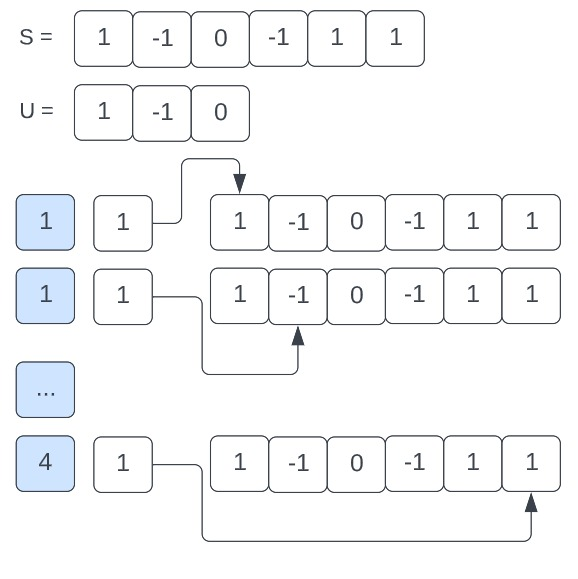
\includegraphics[width=8cm]{exp.jpeg}
    \caption{Posible solución}
\end{figure}
\begin{enumerate}
    \item[3.] Al final, comparar el contador(Caja azul) con $\lceil\frac{|S|}{2}\rceil$  para dar el resultado.
\end{enumerate}
\newpage
\subsection{Algoritmo iterativo}
\begin{algorithm}[H]
    \caption{Secuencia mayoritaria}
    \begin{algorithmic}[1]
        \Procedure{SecMayoritaria}{$S$}
        \State$contador \gets 0$
        \State$i \gets 1$
        \State $U \gets  set(S)$ \Comment Se obtienen los valores únicos de S.
        \While{$i < |U| ~\land~ contador < |S|//2~$} \Comment `//' Quiere decir valor piso
        \State$contador \gets 0$
        \For{$ j \gets 1 ~ \textbf{to} ~ |S|$}
        \If{$S_j = U_i$}
        \State$contador+\gets 1$
        \EndIf
        \State$i+\gets 1$
        \EndFor
        \EndWhile
        \If{$contador > |S|//2$}
        \State \Return{True}
        \Else
        \State \Return{False}
        \EndIf
        \EndProcedure
    \end{algorithmic}
\end{algorithm}
\textbf{Complejidad:} Por inspección de código hay dos ciclos (un \textit{mientras-que} anidado dentro de un ciclo \textit{para-todo}) anidados que, en el peor de los casos, $S$ y $U$ son iguales por tanto $O(|S|^{2}).$ Por otro lado, en caso de que todos los elementos de $S$ sean de un mismo valor, ocurrirá el mejor caso  $\Omega(|S|)$.\\
\textbf{\\Invariante:}
En la primera iteración $i$, el elemento $U_i$ es el elemento con mas ocurrencias.
\begin{enumerate}
    \item \textbf{Inicio:}  $i \gets 1$, la secuencia no esta vacia.
    \item \textbf{Iteración:} $1 \leq i < |S|$, en cada iteración el contador esta aumentando si se cumple que $S_j = U_i$
    \item \textbf{Terminación:} $contador > \frac{|S|}{2}$, se cumple que es una secuencia mayoritaria.
\end{enumerate}
\subsection{Algoritmo por dividir y vencer}
\begin{algorithm}[H]
    \caption{Contar frecuencia}
    \begin{algorithmic}[1]
        \Function{frecuencia}{S,l,r,m}
        \State $count \gets 0$
        \For{$i \gets 1 ~ \textbf{to}~ r, ~ i \gets i+1$}
        \If{$S_i = m$}
        \State $count \gets count +1$
        \EndIf
        \EndFor
        \State \Return{$count$}
        \EndFunction
    \end{algorithmic}
\end{algorithm}
\begin{algorithm}[H]
    \caption{Secuencia mayoritaria recursivo}
    \begin{algorithmic}[1]
        \Procedure{mayoritario}{S,l,r}
        \If{$l = r$ }
        \State \Return{$S_l$}
        \EndIf
        \State $mid \gets (r-l)/2 + 1$
        \State $lm \gets \Call{mayoritario}{S,l,mid}$
        \State $rm \gets \Call{mayoritario}{S,mid+1,r}$
        \If{$lm = rm$}
        \State \Return{$lm$}
        \EndIf
        \State $lc \gets \Call{frecuencia}{S,l,r,lm}$
        \State $rc \gets \Call{frecuencia}{S,l,r,rm}$
        \If{$lc > rc$}
        \State \Return{$lm$}
        \Else
        \State \Return{$rm$}
        \EndIf
        \EndProcedure
    \end{algorithmic}
\end{algorithm}
\textbf{Complejidad:} Relación de recurrencia:
\begin{enumerate}
    \item $T(n) = 2 T(n/2) + O(n), cuando ~ n > 1$
    \item $T(n) = O(1), cuando~ n = 1$
\end{enumerate}
Cuando aplicamos el teorema maestro obtenemos que para el peor caso contamos con $O(nlogn)$.\\
\textbf{\\Invariante:}
Durante los llamados recursivos $lm=rm$
\begin{enumerate}
    \item \textbf{Inicio:}  $l  != r$,  se buscan los mayoritarios en diferentes direcciones.
    \item \textbf{Iteración:} Comparar los mayoritarios  $l->m \land  m->r$ y calcular las ocurrencias de cada uno.
    \item \textbf{Terminación:} Al final, con el valor retornado se procede a validar si $r \geq \lceil\frac{|S|}{2}\rceil$
\end{enumerate}
\end{document}